\documentclass[12pt,a4paper]{article}
\usepackage[utf8]{inputenc}
\usepackage{graphicx}
\usepackage{color}
\usepackage[magyar]{babel}
\usepackage{listings}
\usepackage{float}

\usepackage{enumerate}
\usepackage{tikz}
\usetikzlibrary{shapes,arrows}
\usetikzlibrary{positioning}
\usetikzlibrary{arrows.meta}

\tikzset{
block/.style = {draw, fill=white, rectangle, minimum height=3em, minimum width=3em},
tmp/.style  = {coordinate}, 
input/.style = {coordinate},
output/.style= {coordinate},
pinstyle/.style = {pin edge={to-,thin,black}
}
}
\usepackage[siunitx]{circuitikz} 
\renewcommand{\lstlistingname}{Lista}
\usepackage[
	pdftitle={HA5KFU tanfolyam - Szűrők},
	pdfauthor={HA5KFU Rádióamatőr Klub},
	pdfsubject={HA5KFU tanfolyam},
	pdfcreator={latex},
	pdfkeywords={ },
	pdfpagemode=UseOutlines,
	pdfdisplaydoctitle=true,
	pdflang=hu,
	unicode
]{hyperref}

\pagestyle{plain}
\sloppy
\begin{document}
\begin{center}

\includegraphics[width=300pt,keepaspectratio]{figures/ha5kfu.eps}
\\[0.5cm]
Rádióamatőr tanfolyamot segítő jegyzet, egyelőre kidolgozás alatt \\
Összeállította: Kiss Ádám % Feel free to add yourself
\\[1cm]

{\huge \bfseries Szűrők \\[2cm]}



\end{center}

\renewcommand{\contentsname}{Tartalom}\tableofcontents 
\newpage
\section{Motiváció}

Több jelet szeretnénk átvinni a térben.

\paragraph{Ötlet} Egymásra nem hasonlító jeleket adok ki, a vevő kiszűri azt, amelyiket venni szeretné.

\paragraph{Milyen jelet válasszunk?} A természet lineáris differenciálegyenletek írják le, melyek megoldása $e^{x}$ függvény. A szinuszos függvényeket fel lehet írni "e"-ados alakban $\Rightarrow$ Ha szinuszos jeleket adunk ki, akkor a természet hatásai nem rontják el a függetlenséget.

\paragraph{} Kell valami, ami kiválaszt nekünk néhány szinuszt a végtelen sokból!
\section{Ismétlés}

\paragraph{Induktivitás (lendület)} Gurítsunk egy PET palackot a földön. Ha erőt (feszültséget) fejtünk ki, akkor változik a sebessége.

\paragraph{Kapacitás (magassági energia)} Emeljük fel a PET palackot egy asztalra. Az asztal (szigetelő) miatt nem tud leesni. Ha kivesszük alóla az asztalt (zárlat a föld felé), az induktivitása akadályozza a felgyorsulást, de felgyorsul. (Az esés pillanata nem része a hasonlatnak.)

\subsection{Példa}


Kössünk fel egy PET palackot (\ref{fig:palack}. ábra)! Ha energiát adunk bele (meglökjük), beleng. Ekkor egyébként az impulzusválaszát látjuk. Próbáljuk meg ütemesen ütni. Ha lassan leng a kezünk, nem követi le. Ha gyorsan, akkor se. Van egy frekvencia, amin leng!


\begin{figure}[H]
\begin{center}
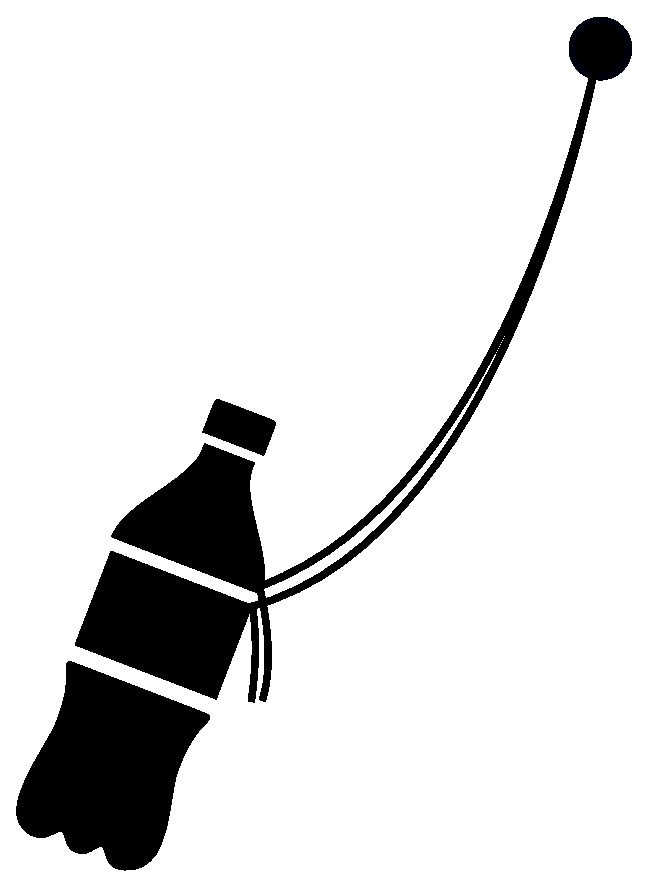
\includegraphics[width=4cm]{figures/szurok_palack.eps}
\caption{Kössünk fel egy PET palackot}
\label{fig:palack}
\end{center}
\end{figure}

\paragraph{Modell} Az induktív lendület (mozgási energia) átalakul kapacitív potenciállá (helyzeti energia).


\begin{figure}[H]
\begin{center}
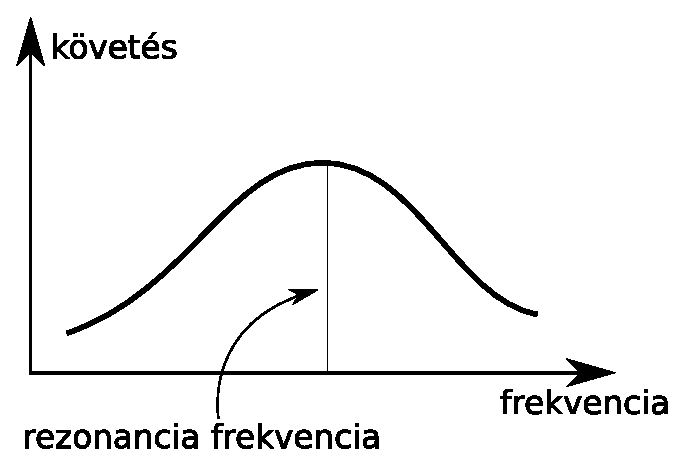
\includegraphics[width=8cm]{figures/szurok_rezonancia.eps}
\caption{Rezonancia frekvencia}
\label{fig:rezonancia}
\end{center}
\end{figure}

Az elrendezés csak egy frekvencia környékén enged át, sáváteresztő jellegű. Ha egyszerre több ember különböző frekvenciával "gerjeszti", akkor is csak a rezonancia frekvencia tud látszani kívülről.

\section{Pár gyakorlati elrendezés}


\begin{figure}[H]
\label{fig:alul}
\centering
\begin{tikzpicture}
	\draw
	(0,0) node(center){} 
	(center) 	to [C] ++(0,-2)  node(btm){}
	(center)		to [L,-o] ++(3,0)
	(-3,0)		to [L,o-] (center)
	(btm)		to [short,-o] ++(3,0)
	(-3,-2)		to [short,o-] (btm)
	%(left1) 		to [short,*-o](-4,0) node[right]{}
	;
	\node [box, right=7cm, yshift=-1cm] (A) {};
    \node [box, right=20mm of A] (B) {};
    \path (A) to [lowpass, name=lpf] (B);
    
    \end{tikzpicture}
\caption{Aluláteresztő szűrő} 
\end{figure}



\begin{figure}[H]
\label{fig:felul}
\centering
\begin{tikzpicture}

	\draw
	(0,0) node(center){} 
	(center) 	to [L] ++(0,-2)  node(btm){}
	(center)		to [C,-o] ++(3,0)
	(-3,0)		to [C,o-] (center)
	(btm)		to [short,-o] ++(3,0)
	(-3,-2)		to [short,o-] (btm)
	%(left1) 		to [short,*-o](-4,0) node[right]{}
	;
	\node [box, right=7cm, yshift=-1cm] (A) {};
    \node [box, right=20mm of A] (B) {};
    \path (A) to [highpass, name=hpf] (B);
    \end{tikzpicture}
\caption{Felüláteresztő szűrő} 
\end{figure}


\begin{figure}[H]
\label{fig:sava}
\centering
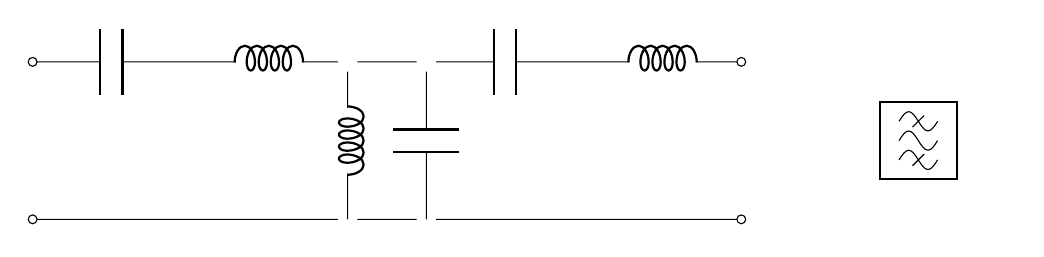
\begin{tikzpicture}

	\draw
	(0,0) node(centera){}
	(1,0) node(centerb){}
	(centera) to [short] (centerb)
		 
	(centera) 	to [L] ++(0,-2)  node(btma){}
	(centerb) 	to [C] ++(0,-2)  node(btmb){}
	
	(btma) to [short] (btmb)
	
	 (-4,0) to [C, o-] ++(2,0)		to [L] (centera) 
	(centerb) to [C] ++(2,0)		to [L,-o] ++(2,0) 
	
	(btma) to [short, -o]  ++(-4,0)
	(btmb) to [short, -o]  ++(4,0)
	;
	\node [box, right=6cm, yshift=-1cm] (A) {};
    \node [box, right=20mm of A] (B) {};
    \path (A) to [bandpass, name=bpf] (B);
    \end{tikzpicture}
\caption{Sáváteresztő szűrő} 
\end{figure}


\begin{figure}[H]
\label{fig:savz}
\centering
\begin{tikzpicture}

	\draw
	(0,0) node(center){}
	
	(center) 	to [L] ++(0,-2) to [C] ++(0,-2)  node(btm){}
	(center)		to [short] ++(-1, 0)  node(topa){}
	(center)		to [short] ++(1, 0)  node(topb){}
	
	(-3 ,0) node(topaa){}
	(3 ,0) node(topbb){}
	
	(topaa) to [short] ++(0,0.5) to [C] ++(2,0) to  [short] (topa)
	(topb) to [short] ++(0,0.5) to [C] ++(2,0) to  [short] (topbb)
	(topaa) to [short] ++(0,-0.5) to [L] ++(2,0) to  [short] (topa)
	(topb) to [short] ++(0,-0.5) to [L] ++(2,0) to  [short] (topbb)
	
	(topaa) to [short, -o]  ++(-1,0)	
	(topbb) to [short, -o]  ++(1,0)
	(btm) to [short, -o]  ++(-4,0)
	(btm) to [short, -o]  ++(4,0)
	;
	\node [box, right=6cm, yshift=-2cm] (A) {};
    \node [box, right=20mm of A] (B) {};
    \path (A) to [bandstop, name=bsf] (B);
    \end{tikzpicture}
\caption{Sávzáró szűrő} 
\end{figure}

\section{Keverők}


\paragraph{Motiváció} Matematikailag levezethető, hogy a szűrők minél több elemet tartalmaznak, annál meredekebben vágnak.

Nagy frekvenciákra így is lehetetlen keskeny szűrőt építeni. Megoldás: toljuk el a jelet!

Ugyanolyan bonyolultságú szűrővel egyre keskenyebb sávot szűrünk!
\newpage

%\renewcommand{\refname}{Irodalomjegyzék}
%\begin{thebibliography}{9}
%
%\end{thebibliography}

\end{document}
